\section{Analisi del problema}

\subsection{Descrizione del problema}
La specifica richiede la realizzazione di due sottopunti:
\begin{enumerate}
    \item Realizzare una libreria con API asincrona utile per recuperare e monitorare informazioni circa treni in viaggio, a partire dall'uso di web API già disponibili in rete.

In particolare la libreria dovrà fornire una API che espone tre metodi asincroni:
\begin{enumerate}
    \item \textbf{getTrainSolutions}: recupera l'elenco delle possibili soluzioni di viaggio fra una stazione di partenza e verso una stazione destinazione, in una specifica data e a partire da una certa ora;
    \item \textbf{getRealTimeTrainInfo}: recupera le informazioni circa lo stato corrente di uno specifico treno;
    \item \textbf{getRealTimeStationInfo}: recupera le informazioni circa lo stato corrente di una specifica stazione.
\end{enumerate}
\item Sviluppare un programma che, usando la libreria sviluppata al punto 1), dato un certo specifico viaggio, permetta di monitorare lo stato dei treni coinvolti, segnalando a che ora è partito/arrivato il treno nelle varie stazioni da cui è partito/a cui è arrivato ed eventualmente possibili ritardi.

Il programma deve fornire una opportuna GUI per identificare/selezionare il viaggio, far partire ed eventualmente bloccare il monitoraggio, e - dato un monitoraggio attivo -  visualizzare nella forma che si ritiene più opportuna l'output del monitoraggio.

È necessario adottare un approccio basato su framework di programmazione ad eventi ad event-loop, come ad esempio Vert.x in Java, ma è possibile utilizzare framework alternativi (es. Node.js in Javascript).

\end{enumerate}

\subsection{API utilizzate}

Per realizzare i 3 metodi asincroni richiesti, ci siamo appoggiati a due API pubbliche già esistenti al fine di reperire le informazioni di nostro interesse. \newline
Le due API Trenitalia utilizzate sono raggiungibili presso \emph{https://www.lefrecce.it/msite/api} e \emph{http://www.viaggiatreno.it/vt{\textunderscore}pax{\textunderscore}internet/mobile}

\begin{itemize}
    \item \textbf{getTrainSolutions}\newline
    \begin{info}[Esempio di chiamata GET su API www.lefrecce.it]\newline

    https://www.lefrecce.it/msite/api/solutions\newline
    ?\textbf{origin}=BOLOGNA CENTRALE\hfill\emph{(stazione di partenza)}\newline
    \&\textbf{destination}=ROMA TERMINI\hfill\emph{(stazione di arrivo)}\newline
    \&\textbf{arflag}=A\hfill\emph{(solo andata / andata e ritorno)}\newline
    \&\textbf{adate}=20/04/2021\hfill\emph{(data partenza)}\newline
    \&\textbf{atime}=15\hfill\emph{(orario partenza)}\newline
    \&\textbf{adultno}=1\hfill\emph{(numero di adulti)}\newline
    \&\textbf{childno}=0\hfill\emph{(numero di bambini)}\newline
    \&\textbf{direction}=A\hfill\emph{(andata o ritorno se arflag=A, sempre A altrimenti)}\newline
    \&\textbf{frecce}=false\hfill\emph{(includere frecce)}\newline
    \&\textbf{onlyRegional}=false\hfill\emph{(includere solo regionali)}
    \end{info}

    \begin{info}[Esempio di chiamata GET su API elaborato]\newline

    http://localhost:8080/train-solution\newline
    ?\textbf{departure}=BOLOGNA CENTRALE\hfill\emph{(stazione di partenza)}\newline
    \&\textbf{arrival}=ROMA TERMINI\hfill\emph{(stazione di arrivo)}\newline
    \&\textbf{date}=20/04/2021\hfill\emph{(data partenza)}\newline
    \&\textbf{time}=15\hfill\emph{(orario partenza)}
    \end{info}

    \begin{figure}[H]
    	\begin{center}
    		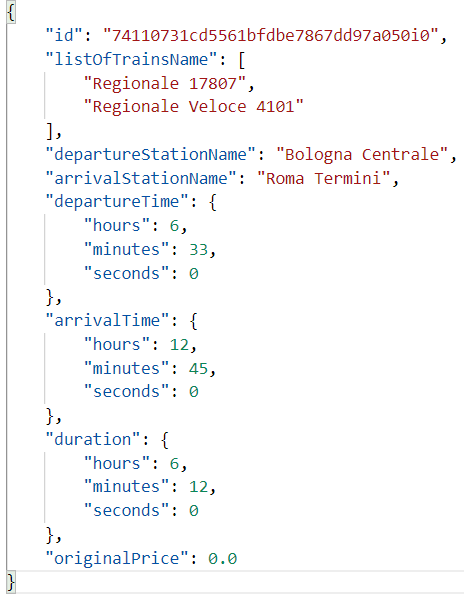
\includegraphics{img/train-solution-json.png}
    		\label{fig:train_solution_json}
    	\end{center}
    \end{figure}

    \item \textbf{getRealTimeTrainInfo}\newline

    \begin{info}[Esempio di chiamata GET su API www.viaggiatreno.it]\newline

    http://www.viaggiatreno.it/vt{\textunderscore}pax{\textunderscore}internet/mobile/scheda\newline
    ?\textbf{numeroTreno}=3922\hfill\emph{(codice del treno da monitorare)}
    \end{info}

    \begin{info}[Esempio di chiamata GET su API elaborato]\newline

    http://localhost:8080/real-time-train-info\newline
    ?\textbf{trainNumber}=3922\hfill\emph{(codice del treno da monitorare)}
    \end{info}

    \begin{figure}[H]
    	\begin{center}
    		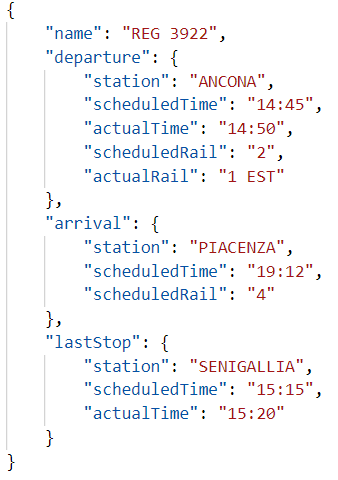
\includegraphics{img/real-time-train-info-json.png}
    	\end{center}
    \end{figure}

    \item \textbf{getRealTimeStationInfo}\newline

    \begin{info}[Esempio di chiamata POST su API www.viaggiatreno.it]\newline

    http://www.viaggiatreno.it/vt{\textunderscore}pax{\textunderscore}internet/mobile/stazione\newline
    ?\textbf{codiceStazione}=S05066\hfill\emph{(codice della stazione da monitorare)}
    \end{info}

    \begin{info}[Esempio di chiamata GET su API elaborato]\newline

    http://localhost:8080/real-time-station-info\newline
    ?\textbf{stationCode}=S05066\hfill\emph{(codice della stazione da monitorare)}
    \end{info}

    \begin{figure}[H]
    	\begin{center}
    		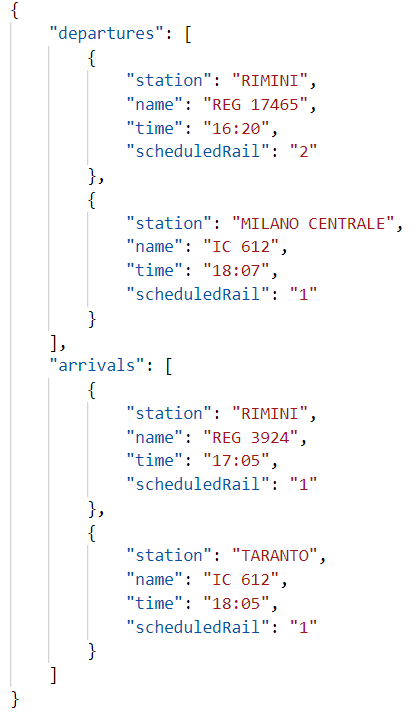
\includegraphics{img/real-time-station-info-json.png}
    		\label{fig:real-time-station-info}
    	\end{center}
    \end{figure}

\end{itemize}
